\documentclass[11pt]{beamer}
\usetheme{Warsaw}
\usepackage[utf8]{inputenc}
\usepackage{amsmath}
\usepackage{amsfonts}
\usepackage{amssymb}
\usepackage{graphicx}
%\author{}
%\title{}
%\setbeamercovered{transparent} 
%\setbeamertemplate{navigation symbols}{} 
%\logo{} 
%\institute{} 
%\date{} 
%\subject{} 
\begin{document}

%\begin{frame}
%\titlepage
%\end{frame}

%\begin{frame}
%\tableofcontents
%\end{frame}

\begin{frame}{Versuchsbeschreibung}
\section{z.B. Widerstand, Teilversuch 4.1}
\subsection{Versuchsbeschreibung}
\begin{itemize}
\item Ohm'sches Gesetz:
\[R=\frac{U}{I}\]
\item $U$ und $I$ gemessen
\end{itemize}
\end{frame}
\begin{frame}{Versuchsaufbau und Durchführung}
\subsection{Versuchsaufbau und Durchführung}
\subsubsection*{Rauschmessungen:}
\begin{figure}
\centering
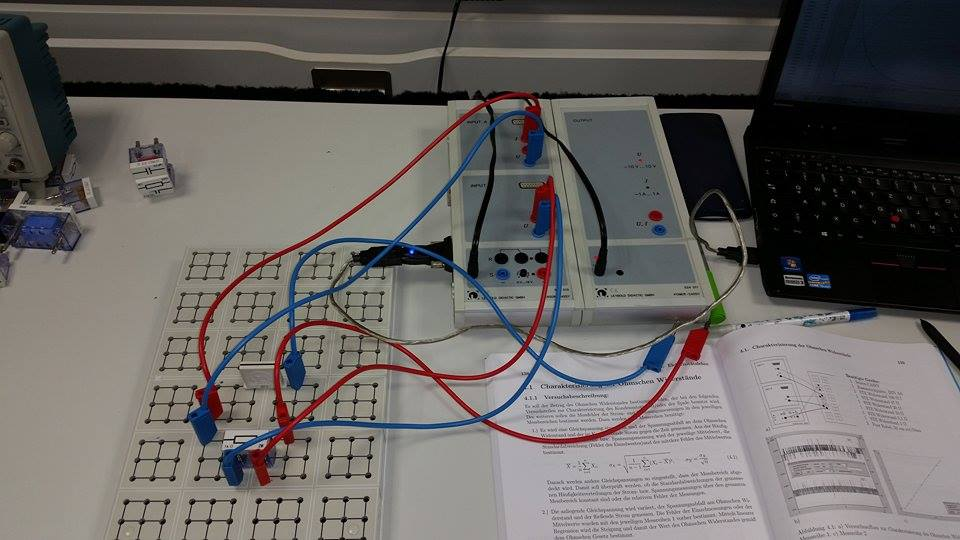
\includegraphics[scale=0.2]{12000155_1207085929316467_1534534399_n.jpg}
\caption{Versuchsaubau}
\end{figure}

\end{frame}
\begin{frame}{Versuchsauswertung}
\subsection{Versuchsauswertung}
\begin{itemize}
\item Mittelwerte von $U$ und $I$ mit stat. Fehler berechnet
\item sys. Fehler aus Herstellerangaben errechnet 
\item Mittelwert für $R$ mit Fehler berechnet
\end{itemize}
\end{frame}
\begin{frame}{Rohdaten}
\subsubsection{Rohdaten}
\begin{figure}
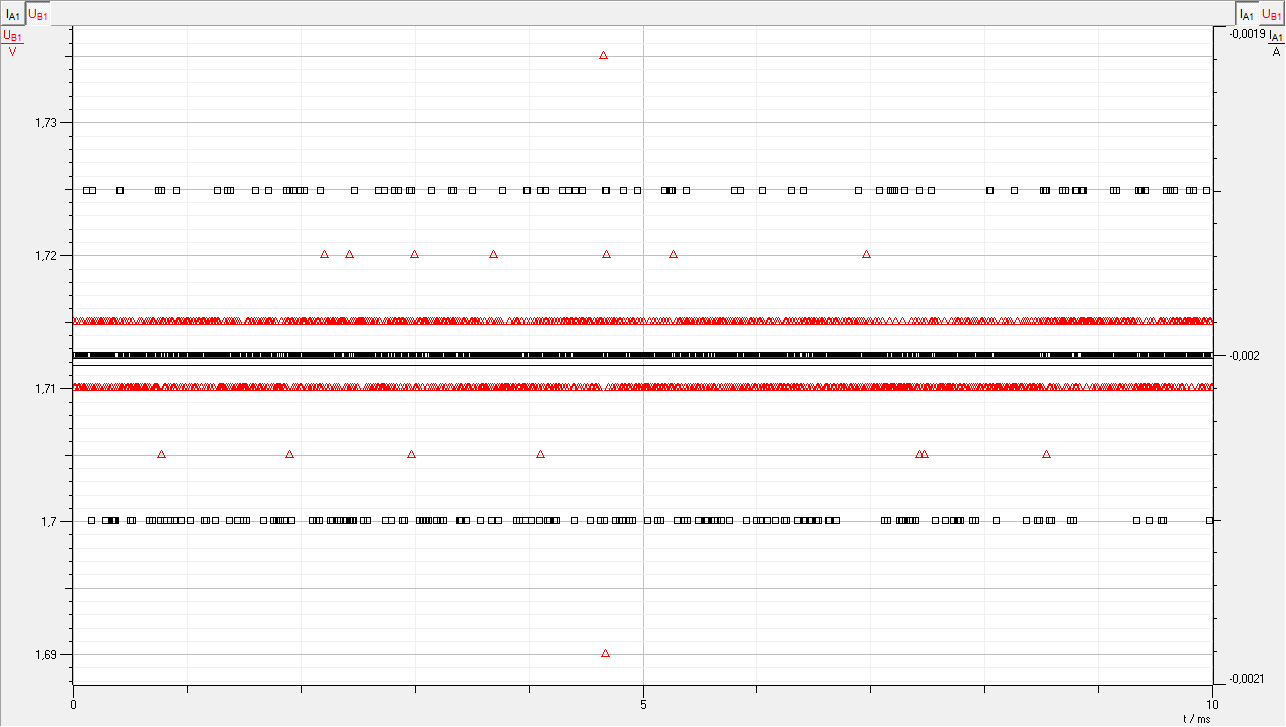
\includegraphics[scale=0.2]{Rauschmessung1.png}
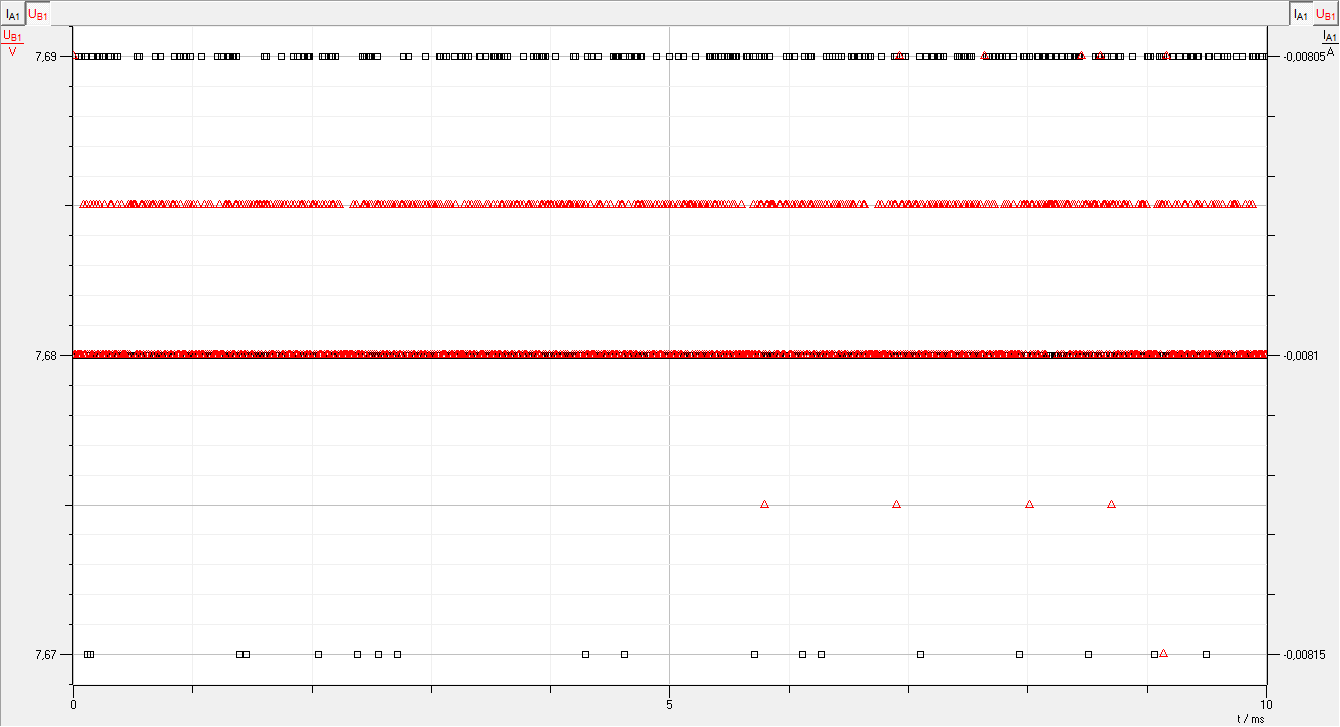
\includegraphics[scale=0.2]{Rauschmessung2.png}  
\caption{Rauschmessungen}
\end{figure}
\end{frame}
\begin{frame}{Analyse}
\subsubsection{Analyse}
\begin{itemize}
\item Formeln:
\begin{align*}
R=\frac{\bar{U}}{\bar{I}} \hspace{2cm} 
\sigma_R=\sqrt{(\frac{1}{\bar{I}})^{2} \cdot \sigma_{\bar{U}}^{2}+(\frac{\bar{U}}{\bar{I}^2})^{2} \cdot \sigma_{\bar{I}}^{2}} \hspace{2cm}\frac{\sigma_R}{R}=\sqrt{(\frac{\sigma_{\bar{U}}}{\bar{U}})^2+(\frac{\sigma_{\bar{I}}}{\bar{I}})^2}
\end{align*}
\item Aus Fehlerrechnungen der stat. Fehlern und sys. Fehlern aus Herstellerangaben des Sensor-Cassy $R$ berechnet
\end{itemize}
\begin{table}[H]\centering
\caption{Ergebnisse}
\begin{tabular}{c|c|c|c|c|c|c}
$\bar{U}$& $\sigma_{\bar{U}}$& $\bar{I}$& $\sigma_{\bar{I}}$& $R$& $\Delta R_{stat}$& $\Delta R_{sys}$ \\ \hline
$1.71V$& $0.00009V$& $0.002A$& $0.00002A$& $855\Omega$& $8.55\Omega$& $233.27\Omega$\\ 
$3.88V$& $0.00008V$& $0.004A$& $0.00002A$& $970\Omega$& $4.85\Omega$& $135.8\Omega$\\ 
$5.82V$& $0.00007V$& $0.006A$& $0.00003A$& $970\Omega$& $4.85\Omega$& $101.84\Omega$ \\
$7.68V$& $0.00009V$& $0.008A$& $0.000026A$& $960\Omega$& $2.4\Omega$& $74\Omega$ \\
\end{tabular} 
\end{table}
\end{frame}
\end{document}